\documentclass{book}
\usepackage[spanish]{babel}
\usepackage[utf8]{inputenc} 
\usepackage[T1]{fontenc}
\usepackage{lmodern}
\usepackage{graphicx}
\usepackage{amsmath}
\usepackage{xcolor}
%\usepackage[natbibapa]{apacite}

\begin{document}
%\chapter{Introdución}
%\chapter{Antecedentes}
\chapter{ Segmentación de imágenes con base en color}
De acuerdo con \cite{bradski2008learning} la visión es la detección de la luz del mundo. Esa luz empieza cuando un rayo emana desde una fuente hacia un objeto. Cuando la luz choca con el objeto, mucha de la luz es absorbida y la que no es absorbida, nosotros la podemos percibir como el color de la luz, de esta manera, la luz reflejada hace su camino hacia nuestra cámara. Esto es de particular importancia para la visión computacional.
		
El modelo más simple de cómo sucede el anterior fenómeno es el de la cámara estenopeica o "pinhole". Una cámara estenopeica se puede imaginar como una habitación sin ventanas en donde la luz únicamente entra por una pequeña apertura en el centro de la pared y que proyecta una imagen dentro de la habitación.

\textcolor{red}{Creo que estos dos párrafos deberían ir dentro de la sección sobre el modelo Pinhole}


\section{El modelo de cámara Pinhole}
Como se había dicho anteriormente el modelo de cámara estenopeica (o pinhole) es el modelo más simple de todos, en donde se considera que la luz entra desde la escena o desde un punto un punto distante, pero sólo un rayo de luz entra desde un punto en particular, este punto es luego “proyectado” sobre una superficie. Como resultado, la imagen en este plano (también llamado plano proyectivo), está siempre en el foco y el tamaño de la imagen se relaciona a la distancia del objeto dado por un sólo parámetro de la cámara: "la distancia focal". La principal diferencia entre el objeto que aparece en una cámara Pinhole, es que la imagen aparece invertida. 
	
El punto dentro del Pinhole es reinterpretado como el centro de proyección. Para este tipo de cámara, la distancia desde la abertura del Pinhole hacia la pantalla, es precisamente la distancia focal. Como puede verse en la Figura 1.\\
	
\begin{figure}
	\centering		
	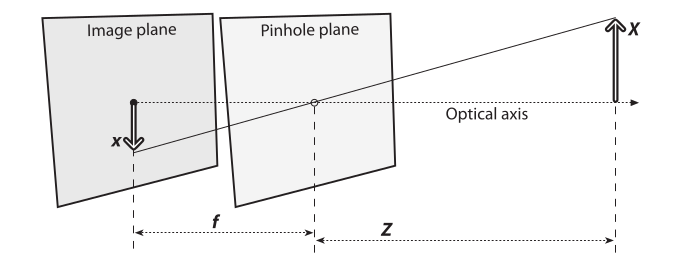
\includegraphics[scale=0.5]{pinhole.png}
	\caption{Esquema del modelo de cámara Pinhole \textcolor{red}{Si copiaste la imagen de algún lado, menciona de dónde la tomaste.}}		
\end{figure}

En la Figura 1, $f$ es representada como la distancia focal de la cámara, $Z$ es la distancia de la cámara al objeto, $X$ es la longitud del objeto, y $x$ es la longitud de la la imagen proyectada en el plano. Dentro de la figura, se pueden ver dos triángulos semejantes los cuales cumplen que $-x/f = X/Z$, o expresado de otra manera:

\[x = -f \frac{X}{Z}\]
	
A fin de obtener ecuaciones equivalentes, pero sin signos negativos (correspondientes a la inversión de la imagen) se propone hacer un rearreglo en el cual se coloca al frente de un centro de proyección al plano proyectivo. Tal y como se ve en la Figura 2.
	
\begin{figure}
	\centering
	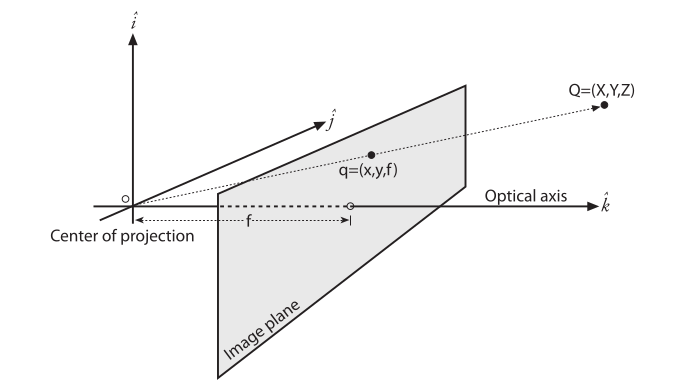
\includegraphics[scale=0.5]{rearreglo_pinhole.png}
    \caption{Rearreglo de una cámara Pinhole \textcolor{red}{Todo debe estar en español}}
\end{figure} 
\textcolor{red}{Revisa la forma de correcta de poner comillas, aunque en textos académicos se estila más usar cursivas en lugar de comillas}
Con este nuevo cambio, el punto en el Pinhole es reinterpretado como ``el centro de proyección'', así cada rayo de luz deja un punto en el objeto distante y se dirije hacia el centro de proyección. El punto de intersección del plano proyectivo y el eje óptico es conocido como \textit{el punto principal}. El nuevo plano de imagen frontal es equivalente al anterior plano proyectivo, el el cual la imagen del objeto distante tiene exactamente el mismo tamaño que en el esquema mostrado en la Figura 1, la diferencia es que en este caso la imagen no queda invertida, por lo tanto la relación de los triángulos quedaría de la siguiente manera: 
\[x/f = X/Z\]

\textcolor{red}{Para poner letras en cursiva usa el comando textit}
Uno podría pensar \textcolor{red}{Se podría pensar} que ``el punto principal'' es equivalente al centro de la imagen, sin embargo, este centro usualmente no está en el eje óptico, es por eso que se introducen dos nuevos parámetros, $c_{x}$ y $c_{y}$ para modelar un posible desplazamiento (perpendicular al eje óptico) del centro de coordenadas en el plano de proyección. El resultado es que un punto Q en el mundo físico cuyas coordenadas son  (X,Y,Z) es proyectado dentro de la pantalla en una localización de pixeles dada por $(x_{screen},y_{screen})$ de acuerdo con las siguientes ecuaciones:

\[x_{screen}=f_{x}(\frac{X}{Z}) \quad,\quad y_{screen}=f_{y}(\frac{Y}{Z})\]	\\

\textcolor{red}{Y aquí dónde entraron $c_x$ y $c_y$}

Nótese que se han introducido dos diferentes distancias focales, la razón es porque generalmente los pixeles son rectangulares.
		
\section{Corrección de la distorsión}
Desafortunadamente una verdadera cámara pinhole no es una muy buena forma de obtener imágenes porque no reune suficiente luz para crear una imagen aproximada a la real. Es por eso que los ojos y las cámaras usan lentes para reunir más luz que la que estaría disponible en un solo punto.

\subsection{Geometría básica proyectiva}
La relación que mapea los puntos $Q_{i}$ en el mundo físico con coordenadas $(X_{i},Y_{i},Z_{i})$ a los puntos en el plano de proyección con coordenadas $(x_{i},y_{i})$ es llamado una $"transformación\;proyectiva"$. Cuando se trabaja con estas transformaciones es conveniente usar $"coordenadas\;homogéneas"$. El plano de imagen es el espacio proyectado y tiene dos dimensiones, con lo que se puede representar puntos en el plano como un vector tridimensional $q=(q_{1},q_{2},q_{3})$ \textcolor{red}{Si tengo un plano, por qué usaría tres dimensiones?}. Una forma de hacer un arreglo con los parámetros que definen a la cámara $f_{x},f_{y},c_{x}\;y\;c_{y} $ dentro de una matriz de 3x3 el cual es llamado matriz de parámetros intrínsecos. La proyección $q$ de los puntos del mundo físico dentro de la cámara es resumida dentro de la 	siguiente forma \textcolor{red}{...del mundo físico en el plano de la imagen se puede calcular como:}.
\[q=MQ\]
donde
\[q=
\begin{bmatrix}
x\\ 
y\\
z 
\end{bmatrix}\;,\;M=
\begin{bmatrix}
f_{x} & 0 & c_{x}\\ 
0     &f_{y}&c_{y} \\
0     & 0 & 1
\end{bmatrix}\;,\;Q=
\begin{bmatrix}
X\\
Y\\
Z
\end{bmatrix}
\]
\subsection{Distorsión de las lentes}
La estimación de los parámetros internos es importante en la calibración de las cámaras \cite{weng1992camera}.


Dada la manufactura y diversos factores, las lentes no son perfectas, es por eso que se introducen dos nuevos conceptos a la distorsión de las lentes, las $"Distorsiones\;radiales"$ y las $"Distorsiones\;tangenciales"$. Las primeras surgen como resultado de la forma de las lentes y las segundas como resultado del proceso de ensamblado de la camara.

\textcolor{red}{Te falta agregar todas tus referencias}
%	\section{Los espacios de color RGB Y HSV}
%	\section{Operadores morfológicos}	
%	\chapter{Estimación de posición y velocidad}
%	\chapter{Implementación}
%	\chapter{Resultados}
%\bibliographystyle{apacite}
\bibliographystyle{ieeetr}
\bibliography{References}
\end{document}
